\chapter{跨域知识图谱的知识表示学习关键技术}
传统的知识图谱嵌入模型通过提取三元组中的事实特征来对实体和关系进行编码。这类模型设计了评分函数,如TransE、RESCAL等,来对嵌入后的三元组进行打分,从而改进了图谱嵌入的效果。然而,在跨域的混合知识图谱的实际应用下,图谱会引入训练数据中不存在的实体和关系。由于传统的嵌入模型不能很好地从训练集中学习到这些组件的特征表示,因此局限性较大。基于规则和归纳推理的方法通常仅集中于表示单个未见部分,而从知识图谱的子图或关系结构特征中学习到的向量表示则忽略了图谱中的隐含语义信息。

为了解决这一问题,本文运用元学习的思想,通过对训练任务的划分和目标场景的模拟,获得对未见实体和关系的特征学习能力。同时,本文将本体也嵌入到低维向量空间中用于辅助图谱表示学习,对未见部分的语义信息补充。在提取了未见关系和未见实体的特征后,为了充分利用已知实体和关系的特征信息,模型采用GNN网络对所有实体和关系统一进行特征更新。本章介绍本文模型涉及到的本体嵌入方法、基于GNN的表示学习方法以及元学习相关的关键技术和代表模型。

\section{跨域知识图谱的知识表示学习定义}
一个知识图谱由众多的事实三元组组成,通常可以定义为\(\mathcal{G} = (\mathcal{E},\mathcal{R},\mathcal{T})\),其中\(\mathcal{E}\)指代所有图谱实体的集合,\(\mathcal{R}\)指代图谱所有关系的集合,\(\mathcal{T}\)指代所有的实体三元组集合,三元组大多遵循RDF等标准进行存储。事实三元组集合中组成三元组的头尾实体和关系均来自于实体集\(\mathcal{E}\)和关系集\(\mathcal{R}\)中,即\(\mathcal{T}=\{(h,r,t) \subseteq \mathcal{E} \times \mathcal{R} \times \mathcal{E}\}\)。
对于传统知识图谱上的链接预测任务,通过给定一个三元组的头结点和关系\((h,r,?)\)或者尾结点和关系\((?,r,t)\)来预测缺失的实体节点\(e \in \mathcal{E}\),使得该缺失的实体节点能构成一个事实三元组\((h,r,t)\),以完成对现有知识图谱的知识补全。为了评估表示学习模型在链接预测任务上的效果,通常会设置两组三元组数据,一组训练三元组\(\mathcal{T}_{support}\)用于对表示学习模型的参数进行学习,另一组测试三元组\(\mathcal{T}_{query}\)包含了训练集中不存在的知识图谱的其他隐藏的事实三元组用于对模型的学习效果进行测试。例如对一个尾结点的预测任务,给定在测试三元组中的一个事实\((h,r,t) \in \mathcal{T}_{query}\),通过模型计算所有可能预测三元组\(\{(h,r,e) | e \in \mathcal{E}, (h,r,e) \notin \mathcal{T}_{support} \cup \mathcal{T}_{query}\}\),如果在所有预测三元组中\((h,r,t)\)的得分越高则说明该表示模型的效果越好。

在跨域知识图谱的训练场景下,本文对传统的知识图谱链接预测任务的定义进行了场景适配。基于跨域知识图谱的现实场景,在源知识图谱上训练的模型需要直接应用在处于低资源环境的目标知识图谱上。由于成本、用户数据隐私等限制,无法将目标知识图谱与源知识图谱进行合并重新训练,因此划分出跨域知识图谱,源域知识图谱包含大量已知事实三元组用于训练,目标域知识图谱作为源域知识图谱子集可能包含未定义的实体和关系用于测试。现给定一个用于训练的源域知识图谱\(\mathcal{G}^{train} = (\mathcal{E}^{train})\),训练的目标是在源域知识图谱上进行模型参数的学习,从而能够将该模型应用在包含未见实体和未见关系的目标域知识图谱上,即\(\mathcal{G}^{test} = (\mathcal{E}^{test},\mathcal{R}^{test},\mathcal{T}^{test}_{support},\mathcal{T}^{test}_{query})\)。跨域知识图谱中的实体集和关系集遵循\((\mathcal{E}^{train} \neq \mathcal{E}^{test},\mathcal{E}^{train} \cap \mathcal{E}^{test} \neq \emptyset)\)及\((\mathcal{R}^{train} \neq \mathcal{R}^{test},\mathcal{R}^{train} \cap \mathcal{R}^{test} \neq \emptyset)\)。其中\(\mathcal{T}^{test}_{support}\)只用于标记测试集中实体与关系的结构,不用于对模型的训练。

\section{本体嵌入关键技术}
本体图是一种特殊的知识图谱,不同于一般的实例知识图谱。本体规定了一系列基本概念之间的语义关系。通常,本体以层次概念为骨架,通过属性来描述概念的语义关系,以表示通用或特定领域的知识。随着知识表示学习的不断发展,传统基于图结构信息进行表示学习的KGE方法在面对跨域知识图谱等场景下,存在一定局限性。因此,越来越多的学者尝试引入本体来补充传统KGE方法的不足,以提高表示学习的效果。例如,从实例视角出发,知识图谱中包含丰富的事实三元组,例如(奥巴马,政治家,美国)。而从本体的角度来看,知识图谱从大量的事实三元组中提取并构建出抽象概念的语义元关系,例如(政治家,领导,国家)。这些本体信息不仅描述实体或关系的限制条件,如属性域和取值范围等,也是对知识图谱语义信息的抽象和集中表示。
\begin{figure}[h]
  \centering
  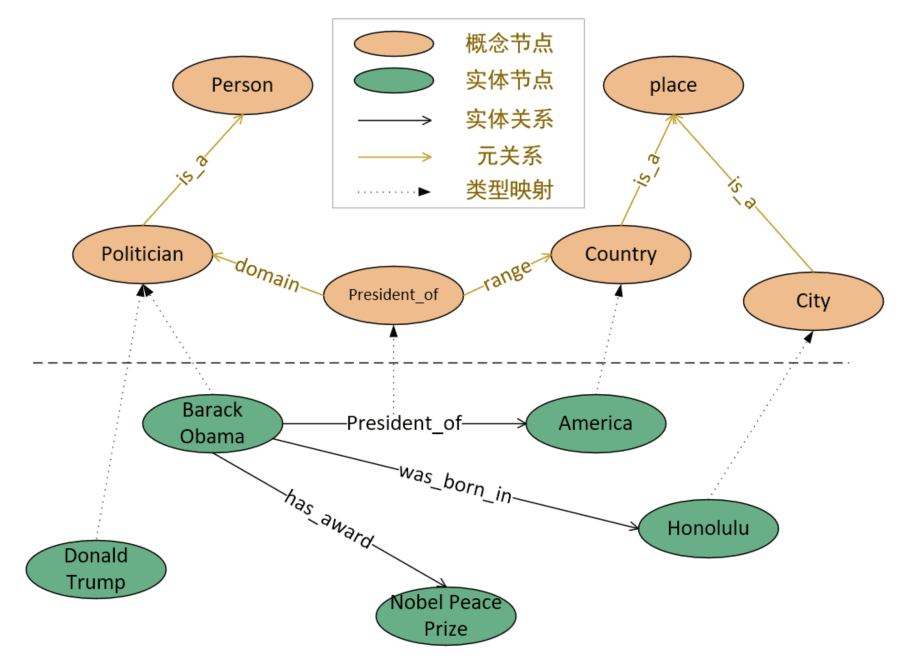
\includegraphics[width=0.6\textwidth]{2-1.png}
  \caption{知识图谱的本体视角和实例视角}
  \label{fig:2-1}
\end{figure}

本体图包含概念和概念间的元关系,通常定义为,其中是概念的集合,是元关系的集合。类似于实体三元组,一个本体三元组(s,r,t)表示概念s,t通过元关系r进行联系。然而,与实例知识图谱复杂多样的关系不同,元关系可进一步分类为传递关系、对称关系、层次关系和其他简单关系\cite{chen2018on2vec}。借鉴于KGE方法的思想,On2Vec\cite{chen2018on2vec}尝试将本体概念和元关系也映射为低纬向量用于本体图的补全。但该模型认为由于本体关系大多具有如传递、对称等特性,不能直接将KGE方法应用在一般的本体图上。例如对称关系r的两个三元组(c$_{1}$,r,c$_{1}$)和(c$_{1}$,r,c$_{1}$),当采用TransE等方法学习嵌入,无法同时兼顾三元组对应的向量满足\(\textbf{c}_{1,r} + \textbf{r} ≈ \textbf{c}_{2,r}\)和\(\textbf{c}_{2,r} + \textbf{r} ≈ \textbf{c}_{1,r}\)。为了解决上述问题,On2Vec通过设置两个特定于关系的投影,以区分同一概念在特定关系头尾的不同编码,如公式\ref{eq:2-1}所示:
\begin{equation}
  S_{d}(T) = || f_{1,r}(\textbf{s}) + \textbf{r} -f_{2,r}(\textbf{t})||,\label{eq:2-1}
\end{equation}
其中\(f_{1,r}\)和\(f_{2,r}\)分别代表了对特定关系r的三元组作为头本体和尾本体不同的投影操作。通过对头部本体和尾部本体分别进行不同的映射,可以很容易地解决上述传递元关系和对称元关系引起的矛盾问题。对于映头尾本体映射操作的选择,On2Vec采用简单的线性变换处理,如公式\ref{eq:2-2}所示:
\begin{equation}
  \begin{aligned} 
    &f_{1,r}(\textbf{s}) = \textbf{M}_{1,r}\textbf{s}, \quad\textbf{M}_{1,r} \in \mathbb{R}^{k \times k}, \\
    &f_{2,r}(\textbf{s}) = \textbf{M}_{2,r}\textbf{s}, \quad\textbf{M}_{2,r} \in \mathbb{R}^{k \times k},
    \end{aligned} \label{eq:2-2}
\end{equation}

特别对于层次关系,On2Vec将层次关系进一步划分为R$_{r}$和R$_{c}$,R$_{r}$关系表示粗略概念被划分为更细致概念的细化关系,而R$_{c}$表示将更细致概念分组为更粗略概念的简略关系。该模型为了使得更细致概念的嵌入紧密地汇聚在一个紧密的邻域内,采用层次模型对层次关系进行单独的处理,对层次关系嵌入的评分函数设置如公式\ref{eq:2-3}所示:
\begin{equation}
  \begin{aligned} 
    S_{hm}(G) = &\sum_{r\in R_{r}} \sum_{s\in C} \sum_{r\in \sigma(s,r)} \omega(f_{1,r}(\textbf{s}) + \textbf{r},f_{2,r}(\textbf{t}))\\
    + &\sum_{r\in R_{c}} \sum_{t\in C} \sum_{r\in \sigma(t,r)} \omega(f_{2,r}(\textbf{t}) -\textbf{r},f_{1,r}(\textbf{s})),
    \end{aligned} \label{eq:2-3}
\end{equation}
其中,\(\omega\)是一个相对于两个参数向量的角度或距离单调递增的函数。On2Vec采用余弦距离进行计算。其中\(\sigma\)是针对于相应层次关系的本体提取操作,对细化关系则寻找所有该关系下的所有尾本体,对简略关系则寻找该关系下的所有头本体。On2Vec扩展了TransE方法,以捕获本体关系的关系属性和层次结构,实现对本体概念和元关系的表示。该方法证明了在本体图上应用知识图谱嵌入方法的有效性。

一些利用本体进行知识表示学习的方法,将本体信息视为实体和关系的附加类型信息。实体使用本体定义的类型进行表示,关系也使用语义类型进行表示。例如,将“马斯克”表示为本体定义的“人类”概念,“特斯拉”则表示为所属“公司”概念。SSE\cite{guo2016sse}模型结合实体的语义类别,将属于同一类别的实体平滑地嵌入到语义空间中。为了更有效地捕捉这些高层本体类型信息带来的限制效果,该模型提出了两种在语义层面对嵌入变量的限制。首先该模型借用拉普拉斯特征映射的算法思想认为,同一个语义类别下的实体的嵌入应该更加相近。例如,对于同属于国家语义的“法国”实体和“意大利”的实体,他们对应的嵌入表示应该更为相似。为此模型为每一个实体设置了一个语义分类矩阵\(W^{(1)}_{ij}\),如果任意两个实体在类型上是相同的,那么该矩阵中对应的值即为1,否则为0。基于该矩阵计算两个实体之间的语义平滑值,如公式\ref{eq:2-4}所示:
\begin{equation}
  \mathcal{R}_{1} = \frac{1}{2} \sum_{i=1}^{n} \sum_{j=1}^{n} \| e_{i} - e_{j} \|_{2}^{2}W^{(1)}_{ij}, \label{eq:2-4}
\end{equation}
其中\(e_{i}\)和\(e_{j}\)指代两个实体i和实体j对应的嵌入表示,通过让两个同类实体的语义平滑值最小,来实现拉普拉斯特征映射的语义限制。其次,该模型还提出一种基于局部线性嵌入的语义约束思想。这种思想不同于拉普拉斯特征映射对数据对局部不变性的设定。基于局部线性嵌入的思想认为,一个实体可以通过其最接近的邻居节点经过一个线性的组合器来近似地表示。例如,“法国”的实体嵌入可以通过其语义相邻的节点,如“中国”、“意大利”等国家节点,通过线性组合的方式来近似地表示。同样,在该语义约束下SSE设置了一个类别邻接矩阵\(W^{(2)}_{ij}\),该矩阵指明实体的连接节点是否是该节点语义范畴内的最邻近节点。然后在该约束下计算实体的语义平滑值,如公式\ref{eq:2-5}所示:
\begin{equation}
  \mathcal{R}_{2} = \sum_{i=1}^{n} \left\| e_{i} - \sum_{e_{j}\in\mathcal{N}(e_{i})}W^{(2)}_{ij}e_{j} \right\|_{2}^{2}, \label{eq:2-5}
\end{equation}
其中\(e_{i}\)和\(e_{j}\)指代两个实体i和实体j对应的嵌入表示,通过使得实体i和所有最邻近节点的线性组合距离最短来实现该猜想的约束。最后,该模型通过在基于距离和基于语义相似度的嵌入模型上加入两种语义约束来提高嵌入表示的效果。实验证明,在语义类别的约束下,表示学习获得了很好的嵌入效果。虽然通过这两种类别信息的约束能够有效引入图谱除结构外的额外知识,但该模型认为单个实体只属于一个类别,忽略了多个类别之间可能的联系,没有完全充分利用好本体的类别语义知识。

TKRL\cite{xie2016representation-TKRL}模型基于传统的翻译模型,并结合本体的实体类型信息,提出了一个基于实体类型的嵌入方法。与SSE模型仅设定实体单一类别不同,TKPL模型认为一个实体可能有多个不同语义层次的类别。并且这些不同层次的类别信息应该被转化到与类别绑定的不同的特征空间中。因此,三元组中的每个实体都应该包含多个实体类型相关的特征信息联合表示。为了获取实体的多类别语义信息,TKPL模型采用所有实体类型转换矩阵的加权和来计算最后的转换矩阵,如公式\ref{eq:2-6}所示:
\begin{equation}
  M = \frac{\sum^{n}_{i = 1}\alpha_{i}M_{c_{i}}}{\sum^{n}_{i = 1}\alpha_{i}}, \alpha_{i} = \left \{\begin{array}{ll}
    1,\quad c_{i} \in C_{r}\\
    0,\quad c_{i} \notin C_{r}
    \end{array} 
    \right.\label{eq:2-6}
\end{equation}
其中n是一个实体所有可能的实体类型数量,\(c_{i}\)指代第i个实体类型,\(M_{c_{i}}\)是该实体类型对应的转化矩阵,\(\alpha_{i}\)是矩阵对应的权重值,最后的\(C_{r}\)指代三元组给定三元组(h,r,t)头实体所有与关系r相连接的可能的实体类型的集合。TKRL引入实体类型信息,并对所有可能的类型信息进行聚合,来增强嵌入模型的学习效果。

为了提高知识表示学习的性能,现有的大多数本体模型在知识嵌入过程中都只包含单一的本体信息,无法实现对所有可用本体信息的无缝嵌入。在现实世界中,知识图谱通常是不完整的,单一的本体信息对补充图谱的作用有限。本文能够在知识嵌入过程中无缝地整合所有可用的本体信息,充分补充图谱,提高复杂场景下的决策能力。同时本文使用了一种简单的本体形式,即RDF Schema(RDFS)中,而那些更复杂的OWL本体可以按照一定的标准转换为RDFS本体。本体可以被用作知识图谱的模式,定义实体类型、关系等。本文将本体表示为\(\mathcal{O} = \{\mathcal{C}, \mathcal{P},\mathcal{T}_{o}\}\),其中\(\mathcal{C}\)是概念节点的集合(即实体类型和实体关系),\(\mathcal{P}\)是属性的集合,\(\mathcal{T}_{o}\)是本体三元组的集合。

\section{基于GNN的跨域知识表示学习关键技术}
图神经网络模型是专门用于处理图数据的模型,可以直接输入一个图网络,并能够很容易地进行节点级别、边级别及图级别的预测任务。CNN模型只能作用在具有相同结构的图像或者特定序列的语音和文字上,而图数据没有固定的形式且邻居节点的也都是无序的,因此CNN模型无法作用在复杂的知识图谱上。相比之下,GNN通过聚合和更新操作,能够学习到图谱结构和节点特征的有效信息。

为了有效地学习图的结构信息和节点特征,并对特征进行嵌入,GNN主要包含了两个部分:聚合函数和更新函数。聚合函数可以将相邻节点的特征进行聚合,并可以使用诸如sum、mean和max等常见操作。一次聚合操作可以提取邻接节点的信息,这些节点距离当前节点为一跳。GNN通常包含多层,每一层都会用上一层的信息进行聚合和传递。因此,n层聚合后传递的信息包含了n层邻接节点的结构信息和节点本身的特征信息。每层的特征聚合函数,如公式\ref{eq:2-7}所示:
\begin{equation}
  h_{v}^{k} = \sigma(W_{k} \sum \frac{h_{u}^{k-1}}{|N(v)|} + B_{k}h_{v}^{k-1}) \quad where \quad k = 1, ..., k-1 \label{eq:2-7}
\end{equation}

从公式可以看出,每层包含两个部分信息。首先\(W_{k}\sum\frac{h^{k-1}_{u}}{|N(v)|}\)表示邻接点特征的聚合操作,而后一部分是上一层聚合特征和权重参数的乘积。最后,这两部分特征通过激活函数更新,完成节点特征输出。在GNN模型中,聚合操作没有区分邻接节点的重要性,而是进行了简单的池化操作。

基于GNN的另外一种改进方向集中于对图结构关系表示的补充上。图神经网络关注节点特征的聚合和更新操作,但在信息传递的过程中,图的关系结构仅用于指明邻接点,关系特征未参与节点的更新过程。为了增加关系信息对节点的影响,R-GCN在每层节点特征计算中引入了邻接点间的对应关系,更新函数如公式\ref{eq:2-8}所示:
\begin{equation}
  h_{i}^{l+1} = \sigma \left( \sum_{r\in\mathcal{R}} \sum_{j\in\mathcal{N}_{i}^{r}} \frac{1}{c_{i,r}}W_{r}^{l}h_{j}^{l} + W_{0}^{l}h_{i}^{l}\right), \label{eq:2-8}
\end{equation}

与GNN对邻接点特征聚合的操作不同,R-GCN引入了关系特定的转换。这种转换取决于边的类型和方向。为了确保第l层的节点表示可以受到相应层次的表示的影响,R-GCN在基础的图关系上为每个节点添加了一个自连接的特殊关系。如图\ref{fig:2-2}所示,在R-GCN中每层对一个实体节点(红色块表示)进行特征生成的过程中,首先从邻接点获取特征(蓝色块表示)并根据该节点与邻接节点的关系类型进行特征转换得到该种关系对应的表示(绿色块表示),其中关系类型分别由入关系、出关系以及自循环关系组成。然后将所有关系转换后的邻接节点信息累加求和,并通过一个如ReLU的激活函数即可获得该节点本层的输出表示。相比于R-GCN,近期提出的CompGCN在R-GCN模型的基础上进一步引入了注意力机制,针对每种边类型和方向分别进行了注意力计算以加强对重要信息的关注。而且在计算效率方面,它减少了每个节点的嵌入大小并减少了依赖于固定卷积核的计算量,因此更适合于大规模图数据。
\begin{figure}[h]
  \centering
  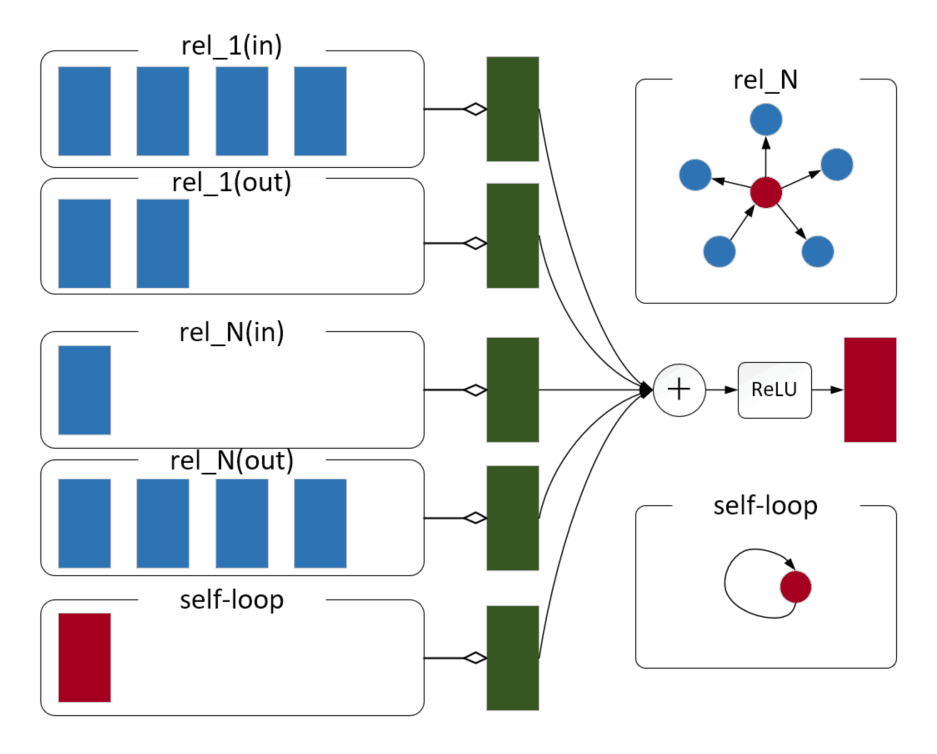
\includegraphics[width=0.8\textwidth]{2-2.png}
  \caption{R-GCN的特征传递}
  \label{fig:2-2}
\end{figure}

随着图卷积网络被广泛应用于图数据处理,它本身的能力也已经可以用于跨域知识表示学习。例如,INDIGO\cite{liu2021indigo}模型使用实体三元组与GNN的内层和外层的特征向量元素之间的一对一对应关系对知识图谱进行编码,并避免了额外的打分函数,充分利用了GNN的特征聚合能力。其他方法如Zhao\cite{zhao2020attention}等人通过基于注意力的图网络聚合未见关系的邻接结构特征,来作为未见关系的表示。但这些方法要么专注于传统的知识图谱表示学习领域,要么通过结构信息对未见的实体或关系进行嵌入,忽略了其他的语义信息。本文通过全局本体信息的嵌入表示,在加强知识引入的同时,借助关系的位置结构信息来训练一个兼顾两种未知部分的基于GNN的表示学习模型。

\section{元学习训练方法}
元学习最普适性的算法思想可以理解为“learning to learn”,它通过多个学习任务的训练来改进学习算法,而传统的机器学习算法则是在多个数据实例上进行模型的学习。

传统的机器学习方法会设置一个训练集\(\mathcal{D} = \{(x_{1},y_{1}),...,(x_{N},y_{N})\}\),例如样本对(输入的图片,图片的标签)。而元学习的目的是训练出一个模型函数\(y = f_{\theta}(x)\),通过训练来获得其中的参数\(\theta\),求解公式如公式\ref{eq:2-9}所示:
\begin{equation}
  \theta^{*} = \underset { \theta } { \operatorname { arg } \operatorname { min } }\mathcal{L}(\mathcal{D};\theta,\omega) \label{eq:2-9}
\end{equation}
其中的\(\mathcal{L}\)是一个损失函数来计算真实标签与模型预测标签之间的误差,\(\omega\)指代了模型如何学习的假设,例如如何为参数\(\theta\)选择合适的优化器或者为\(f\)选择函数类型等。传统的机器学习方法实现过程中,该部分由研究者手动设置。模型的泛化性能则通过评估模型在已知标签上的测试集测试来衡量。传统的机器学习假设是模型的优化是对每个训练集\(\mathcal{D}\)从头开始执行,模型如何学习的设定是预先指定的,这些设定将极大地影响模型的准确性和数据效率等性能指标。元学习试图通过学习学习算法本身来改进这些指标,而不是假设学习算法是预先指定或者固定的。此外元学习从任务的分布中学习,而不是从头开始。

元学习“learning to learn”的思想精髓可以看做一个包含内外两层的双层优化问题,双层优化\cite{stackelberg1952theory}指代的是层次优化问题,其中一个优化包含另一个优化作为约束\cite{franceschi2018bilevel}\cite{sinha2017review}。经典的内外双层模型的算法如MAML,其算法流程如算法\ref{alg:meta}所示:
\begin{algorithm}
  \KwData{\(p(\mathcal{T})\):distribution over tasks}
  \KwData{\(\alpha,\beta\) step size hyperparameters}
    randomly initialize \(\theta\) \\
    \While{not done}{
    Sample batch of tasks \(\mathcal{T}_{i} \thicksim p(\mathcal{T})\)
    \For{\(\mathcal{T}_{i}\)}{
      Evaluate \(\nabla_{\theta}\mathcal{L}_{\mathcal{T}_{i}}(f_{\theta})\) wtih respect to K examples \\
      Compute adapted parameters with gradient descent:\(\theta^{'}_{i} = \theta - \alpha\nabla_{\theta}\mathcal{L}_{\mathcal{T}_{i}}(f_{\theta})\)
    }
    Update \(\theta \leftarrow \theta - \beta\nabla_{\theta} \sum_{\mathcal{T}_{i} \thicksim p(\mathcal{T})}\mathcal{L}_{\mathcal{T}_{i}}(f_{\theta^{'}})\)
  }
  \caption{Model-Agnostic Meta-Learing}\label{alg:meta}
  \end{algorithm}

  在该视角下,元学习任务可以通过公式\ref{eq:2-10}所示来规范化:
\begin{equation}
  \omega ^ { * } = \underset { \omega } { \operatorname { arg } \operatorname { min } } \sum_{i=1}^{M} \mathcal{L} ^ { \text { meta } } ( \mathcal{D} _ { \text { source } } ^ { \text { val } ( i ) } ; \theta ^ { * ( i ) } , \omega ), \label{eq:2-10}
\end{equation}
\begin{equation}
  s.t. \qquad \theta ^ { * ( i ) } ( \omega ) = \underset { \theta } { \operatorname { arg } \operatorname { min } } \mathcal{L} ^ { \text { task } } ( \mathcal{D} _ { \text { source } } ^ { \text { train } ( i ) } ; \theta , \omega ), \label{eq:2-11}
\end{equation}
其中\(\mathcal{L} ^ { \text { meta } }\)和\(\mathcal{L} ^ { \text { task } }\)分别指代外层的优化目标和内层的优化目标,例如在分类任务下的交叉熵。但是这两层的优化级别并不对称,内层优化在基于外层参数\(\omega\)的优化过程中不能对\(\omega\)进行修改。公式中\(\omega\)可以指代如非凸优化\cite{finn2017model}的内层模型的初始化参数或其他可学习的超参数。因此,元学习的整个训练流程分为两层优化:内层模型首先接收外层模型的参数\(\omega\),然后根据自己的任务在该任务的训练集上进行训练,最终在该任务的测试集上计算出损失函数。接下来,外层模型使用内层模型计算出的损失函数对参数\(\omega\)进行更新,使得内层函数的损失达到最优。元学习的思想即通过外层模型的训练,学习到内层模型一个更好的设定,以便让内层模型更好地完成各种任务。

如前所述,内层模型需要特定训练集和测试集以针对面向的问题进行训练。以任务为训练单位的设定是元学习方法不同于传统机器学习方法的一个特点。从训练任务的角度来看,元学习的目标是学习出一种通用的学习算法,这些算法能够在新任务上获得更好的表现。内层模型可以视为使用外层模型参数的传统机器学习算法,其数据集为\(\mathcal{D} = (\mathcal{D}^{train}, \mathcal{D}^{val})\),针对单个任务的损失函数即为\(\mathcal{L}(\mathcal{D};\omega) = \mathcal{L}(\mathcal{D}^{val};\omega^{*}(\mathcal{D}^{train},\omega),\omega)\)。在实际应用中,通常只有一个训练集和测试集。因此,一般会从源训练集中抽样出一组任务用于进行训练。这些任务的训练集和测试集被称为support集和query集,以避免与最终模型训练后进行评估的测试集混淆。

本文旨在跨域知识图谱上进行知识表示的相关研究,并尝试解决在含有未见部分的目标域知识图谱上的链接预测任务。经典的知识图谱表示学习的链接预测任务采用的数据集会设置一个训练集和测试集,测试集中不包含新的实体和关系。因此,本文采用现有数据集中符合问题条件的测试集进行采样,并借鉴元学习“learning to learn”的思想,将这些数据抽取为任务进行训练和测试。从这些训练任务上学习到能够处理未知组件的知识表示方法。

\section{本章小结}
本章首先介绍了跨域知识图谱及问题的定义,强调了跨域知识表示学习中新的实体和关系对传统知识表示学习的影响。为了能够将本体信息用于到知识表示中,介绍了使用本体嵌入的基本方法和代表性的一些应用模型。本体的向量表示,能够为实例图谱的实体和关系提供较为完整的语义信息补充。同时,本文希望通过结合GNN模型对邻接实体和关系的特征进行学习,在第三部分介绍了GNN在知识图谱的知识表示学习上的应用及基于GNN的改进的一些模型方法。最后介绍了元学习相关的思想、原理及方法,为后续模型的任务划分及训练流程提供理论支撑和参考。